%% The LaTeX project Prassble
%% main.tex: the main contents of your document
%%
%% -------------------------------------------------------------------------------------------
%% Copyright (c) 2025 by Grass (GrassGlass) <shaohong00002 at gmail dot com>
%% -------------------------------------------------------------------------------------------
%%
%% This work may be distributed and/or modified under the
%% conditions of the LaTeX Project Public License, either version 1.3
%% of this license or (at your option) any later version.
%% The latest version of this license is in
%%   http://www.latex-project.org/lppl.txt
%% and version 1.3 or later is part of all distributions of LaTeX
%% version 2005/12/01 or later.
%%
%% This work has the LPPL maintenance status `author-maintained'.
%%
%% This work consists of all files listed in README
%%
\ExplSyntaxOn
\AtEndDocument { \benchmark_toc: }
\benchmark_tic:
\ExplSyntaxOff
\documentclass[11pt, a4paper]{book}
% \def\ColourTheme{BnW}
%% The LaTeX project Prassble
%% preamble.tex: the preamble of Prassble
%%
%% -------------------------------------------------------------------------------------------
%% Copyright (c) 2025 by Grass (GrassGlass) <shaohong00002 at gmail dot com>
%% -------------------------------------------------------------------------------------------
%%
%% This work may be distributed and/or modified under the
%% conditions of the LaTeX Project Public License, either version 1.3
%% of this license or (at your option) any later version.
%% The latest version of this license is in
%%   http://www.latex-project.org/lppl.txt
%% and version 1.3 or later is part of all distributions of LaTeX
%% version 2005/12/01 or later.
%%
%% This work has the LPPL maintenance status `author-maintained'.
%%
%% This work consists of all files listed in README
%%
% Preamble
% We split the package loading and package option setting, because it's not a good idea to mix them, apparently: https://tex.stackexchange.com/a/745011/383565

% Packages
  % Encodings
  \usepackage[utf8]{inputenc}
  \usepackage[T1]{fontenc}
  % Language
  \usepackage[UKenglish]{babel} 
  % % Indentation
  %   % See posts: https://tex.stackexchange.com/a/39232/383565 and https://tex.stackexchange.com/a/39228/383565
  %   \usepackage{indentfirst}

  % Named colors
  \PassOptionsToPackage{dvipsnames, table}{xcolor} 
    % The table option of xcolor loads the colortbl package, in order to use the tools for coloring rows, columns, and cells within tables.

  % Tables
  \usepackage{array, booktabs, multirow, cellspace}

  % Figures
  \usepackage{graphicx}
  \graphicspath{{\CurrentFilePath/../figures/}} 
  \usepackage{caption, subcaption, float}

  % Math stuff
  \usepackage{amssymb, mathrsfs}
  \usepackage{mathtools, mleftright, nicematrix}
  \usepackage{intexgral}
    % prerequisites for \hatt command and \reallywidehat
    \usepackage{scalerel, stackengine}
    \usepackage{verbatimbox} % For \addvbuffer

  % % Sciences
  % \usepackage{siunitx}

  % Diagrams
  \usepackage{tikz, pgfplots}
  \usetikzlibrary{cd}
  \pgfplotsset{compat=1.18}

  % enumeration
  \usepackage[shortlabels,inline]{enumitem}
  \usepackage{eqparbox}

  % Margins and line spacing
  \usepackage[margin = 1.25in]{geometry}
  \geometry{
    bottom=15mm}
  \usepackage{setspaceenhanced, parskip}
  \onehalfspacing

  % Page formatting
  \usepackage[pagestyles]{titlesec}
  \usepackage{lmodern, microtype}
    % default colour theme
    \ifundef{\ColourTheme}{\gdef\ColourTheme{colourful}}{}

  % Colored boxes
  \usepackage[skins, breakable, minted]{tcolorbox}
    % Required for autowidth = lower 
    \usepackage{varwidth}
  \setminted{%
    ,escapeinside = ⵌⵌ
    % The characters afterwhich a linebreak can occur:
      % The backslashes are there only to escape the square brackets; the symbols "[" and "]" are the ones afterwhich a linebreak can occur. The \[\] is not indicating display mathmode.
      ,breakafter = \[\]()
  }
  \usepackage{keytheorems}

  % Externalisation 
  % \usepackage{robust-externalize}

  % Refer
  \usepackage{soul} % for special underlining of hyperlinks --- descenders are omitted
  \PassOptionsToPackage{hyphens}{url}
  \usepackage{hyperref}
  \usepackage{zref-titleref}
  \usepackage{zref-clever}
  \usepackage{zref-xr}

% Custom setup

  % Easy input of files
  %% The LaTeX project Prassble
%% Input_macro.tex: an original command \Input for easy input of files.
%%
%% -------------------------------------------------------------------------------------------
%% Copyright (c) 2025 by Grass (GrassGlass) <shaohong00002 at gmail dot com>
%% -------------------------------------------------------------------------------------------
%%
%% This work may be distributed and/or modified under the
%% conditions of the LaTeX Project Public License, either version 1.3
%% of this license or (at your option) any later version.
%% The latest version of this license is in
%%   http://www.latex-project.org/lppl.txt
%% and version 1.3 or later is part of all distributions of LaTeX
%% version 2005/12/01 or later.
%%
%% This work has the LPPL maintenance status `author-maintained'.
%%
%% This work consists of all files listed in README
%%
\ExplSyntaxOn
% Easy input of files; \Input{#2} is \input{#2} but with the file path taken relative to
  % 1. the directory preamble, if \Input is used before \begin{document}
  % 2. the parent directory of the folder preamble (which in this case is the directory Prassble), if \Input is used after \begin{document}
  % 3. \CurrentFilePath, if (at anywhere) the starred variant \Input* is used
% \Input[#1]{#2} has the optional argument #1, which can prepend a file path #1 (folder_1/folder_2/.../folder_n) to the file path #2. That is, \Input[#1]{#2} = \input{#1#2}. But, #1 can also be a 'keyword' that causes the corresponding file path (defined with \KeywordforInput) to be prepended (instead of #1 itself), as well as cause some code (stored in \g_Prassble_Input_prepend_#1_tl and \g_Prassble_Input_append_#1_tl) to be possibly executed.
%* TLDR: \Input[ <keyword / file path to prepend> ]{ <file path relative to directory 'preamble' or '../preamble'> }
\clist_new:N \l__Prassble_files_to_be_input_clist
\seq_new:N \g__Prassble_Input_keywords_seq
\tl_new:N \g_Prassble_Input_prepend_tl
\tl_new:N \g_Prassble_Input_append_tl
\tl_new:N \g_file_directory_to_be_used_tl
\tl_new:N \g_Prassble_path_to_preamble_folder_tl
\tl_new:N \g_Prassble_path_to_Prassble_folder_tl
\tl_new:N \l__Prassble_relative_path_to_prepend_tl
% Set the directory to be the folder 'preamble' in the preamble.
  \tl_gset:Ne \g_Prassble_path_to_preamble_folder_tl {\CurrentFilePath/../../} %* The number of /../ here depends on where Input_macro.tex is placed inside the folder preamble
  \tl_gset:Ne \g_Prassble_path_to_Prassble_folder_tl {\g_Prassble_path_to_preamble_folder_tl../}
  \tl_set_eq:NN \g_file_directory_to_be_used_tl \g_Prassble_path_to_preamble_folder_tl
% Set the directory to be '../preamble' in the document body.
  \AtEndPreamble{\tl_gset_eq:NN \g_file_directory_to_be_used_tl \g_Prassble_path_to_Prassble_folder_tl}

\makeatletter
% Putting the core \Input code in a general function \__Prassble_Input@core:nnnn so that other commands similar to \input (e.g. \inputcode) can also be transformed accordingly (e.g. to \InputCode).
\cs_new:Npn \__Prassble_Input@core:nnnn #1#2#3#4 {
  % If the starred variant \Input* is used, go to the directory \CurrentFilePath.
    \bool_if:nT {#1} 
      {
        \tl_set:Nn \g_file_directory_to_be_used_tl {\CurrentFilePath}
      }
  % Test whether #2 is a keyword
    \seq_if_in:NeTF \g__Prassble_Input_keywords_seq {#2} 
      {
        % If so, set the corresponding 
          % path to prepend
          % code to prepend
          % code to append
        \tl_if_empty:cF {g__Prassble_Input_relative_path_to_prepend_#2_tl} {
          \tl_put_right:cn {g__Prassble_Input_relative_path_to_prepend_#2_tl} {/}
        }
        \tl_set_eq:Nc \l__Prassble_relative_path_to_prepend_tl {g__Prassble_Input_relative_path_to_prepend_#2_tl}
        \tl_set_eq:Nc \g_Prassble_Input_prepend_tl {g_Prassble_Input_prepend_#2_tl}
        \tl_set_eq:Nc \g_Prassble_Input_append_tl {g_Prassble_Input_append_#2_tl}
      } 
      {
        % Otherwise, #2 is a file path that is to prepended as-is
        \tl_if_empty:nF {#2} {
          \tl_set:Nn \l__Prassble_relative_path_to_prepend_tl {#2/}
        }
      }
    % \input the files approperiately
    \clist_set:Nn \l__Prassble_files_to_be_input_clist {#3} 
    \clist_map_inline:Nn \l__Prassble_files_to_be_input_clist 
        {
            \tl_use:N \g_Prassble_Input_prepend_tl
            #4{\g_file_directory_to_be_used_tl\l__Prassble_relative_path_to_prepend_tl##1}
            \tl_use:N \g_Prassble_Input_append_tl
        }
  % Reset the path to prepend
    \tl_clear:N \l__Prassble_relative_path_to_prepend_tl
  % Reset the keyword
  \tl_clear:N \l__Prassble_relative_path_to_prepend_tl
  \tl_clear:N \g_Prassble_Input_prepend_tl
  \tl_clear:N \g_Prassble_Input_append_tl
}
\NewDocumentCommand{\Input}{ s O{} m }{
  \__Prassble_Input@core:nnnn { #1 } { #2 } { #3 } { \input }
}
\makeatother
\ExplSyntaxOff
  \KeywordForInput{HW}{files/homework}                %*
  
  % Math stuff
  \Input[math]{%
    ,general_math.tex%
    ,specific_math.tex%
    }
  
  % enumeration
  \Input{enumeration.tex}

  % Custom symbols (\eeveeKawaii, \TikZ, etc)
  \Input{custom-symbols.tex}
  
  % page formatting
  \definecolor{HeaderColour}{RGB}{0,82,155}            %*
  \author{Author}                                     %*
  \def\CourseName{\textlangle Course Name\textrangle} %*
  \newcounter{HWNumber}                               %*
  \Input{page-formatting.tex}

  % Colored boxes
    % Nonlistings
    \Input[environments/box_styles/nonlistings]{%
      ,theoremstyles.tex%
      ,commands/modified_commands/newkeytheorem.tex
      ,commands/newcommands/InputKeyword_HW-in-Main.tex
      ,../lengths_and_counters.tex%
    }
    \Input[environments/derived_environments]{%
      ,lengths.tex%
      ,nonlistings.tex%
    }
    % Listings
    \Input[environments/box_styles/listings/commands/newcommands]{%
      ,all_short_names.tex%
      ,new_variables.tex%
      ,name_converters.tex%
    }
    \Input[environments/box_styles/listings/commands/modified_commands]{%
      ,../../codestyles.tex%
      ,NewInputListing.tex%
      ,NewListing.tex%
    }
    \Input{environments/derived_environments/listings.tex}

  % Refer
  \Input{external_hyperlink_format.tex}
  \hypersetup{
    ,colorlinks=true
    ,linkcolor=blue
    ,filecolor=magenta
    ,urlcolor=cyan
    }

  % Other
  \Input{other.tex}
  \AddToHWEnvList{table,figure}                       %*
  \newcommand{\HWInMainHeader}{\subsection{Homework \#\arabic{HWNumber}}}                                        %*
\begin{document}
\frontmatter
%
%% The LaTeX project Prassble
%% maintitlepage.tex: a nice coverpage for main.tex
%%
%% -------------------------------------------------------------------------------------------
%% Copyright (c) 2025 by Grass (GrassGlass) <shaohong00002 at gmail dot com>
%% -------------------------------------------------------------------------------------------
%%
%% This work may be distributed and/or modified under the
%% conditions of the LaTeX Project Public License, either version 1.3
%% of this license or (at your option) any later version.
%% The latest version of this license is in
%%   http://www.latex-project.org/lppl.txt
%% and version 1.3 or later is part of all distributions of LaTeX
%% version 2005/12/01 or later.
%%
%% This work has the LPPL maintenance status `author-maintained'.
%%
%% This work consists of all files listed in README
%%
\colorlet{titlepagecolor}{NavyBlue}
\colorlet{textcolor}{white}
\begin{titlepage}
    \newgeometry{left=7.5cm} %defines the geometry for the titlepage
    \pagecolor{titlepagecolor}
    \noindent
    \large
    \color{textcolor}
    \Huge Decoration\normalsize\\
    \makebox[0pt][l]{\rule{1.3\textwidth}{1pt}}
    \par
    \noindent
    \textbf{\textsf{Author}}{\textsf{}}
    \vfill
    \noindent
    {\huge\textsf{Document Name}}
    \vskip\baselineskip
    \noindent
    \textsf{Other information (e.g. 1st January 2025--\today)}
\end{titlepage}
\restoregeometry % restores the geometry
\nopagecolor% Use this to restore the color pages to white
\thispagestyle{empty} % use this if you're not writing anything between the titlepage and the toc
%
\addtocontents{toc}{\protect\thispagestyle{empty}}
\tableofcontents
\thispagestyle{empty}
\newpage
\setcounter{page}{1}
%
\mainmatter
\chapter{Name of First Chapter}
This document can be used as a compilation of all work one produces in a course. For instance, it may include self-proofs of given theorems and all homework submissions.
%
\section{Name of First Section}
\Input{files/chapters/ch1/sec1.tex}
%
\section{Name of Second Section}
\subsection{Theorems}
\begin{theorem}
    This is the second theorem.
\end{theorem}
\begin{proof}
    This is the proof to the second theorem.
\end{proof}
\begin{corollary}(standalone)
    This is a corollary that is trivial enough for the proof to be left unstated. As such, we use the \TeXinline{type in thmgroup = standalone} option.
\end{corollary}
\subsection{Exercises}
\begin{exercise}\label{ex:1.2}
    Another exercise.
\end{exercise}
\begin{code}{Text}
    Some code as part of the answer to ⵌ\zcref{ex:1.2}ⵌ.
\end{code}
\begin{answer}
    The answer to \zcref{ex:1.2}.
\end{answer}
These are some hyperlinks with \TeXinline{zref-clever}: \zcref{ex:1.1}, \zcref{ex:1.2}, \zcref{ex:H.1.1}, \zcref{ex:H.1.2}, \zcref{ex:H.1.3}. We can also reference theorems: \zcref{thm:1.1}. Furthermore, \extref{https://www.google.com/search?q=external+link}{external links} are nicely formatted with the \TeXinline{\extref{ⵌ\textlangleⵌURLⵌ\textrangleⵌ}{ⵌ\textlangleⵌlink nameⵌ\textrangleⵌ}} command.
\newpage
This is the second page.

\newpage
This is the third page.
%
%
\chapter{Name of second chapter}
%
\section{Name of first section}
We insert an example figure here:
\begin{figure}[H]
    \centering
    \includegraphics[page=2]{Three_Planes_Orthogonal_Complements.pdf}
    \caption{Example captions.}
    \label{fig:Three_Plane_Orthogonal_Complements}
\end{figure}
\subsection{Theorems}
\subsection{Exercises}
\begin{exercise}
    This is the first exercise of the second chapter.
\end{exercise}
\backmatter

\end{document}